\chapter{Theoretical foundations}
\label{chap:theoretical-foundations}

\section{Probability theory}
\label{sec:some-probability}

Our computations are based on fundamental probability theoretic considerations. We therefore introduce some important concepts, where we rely on established notation (i.e. we use $\p{}$ to denote probabilities, $\E{}$ for expected values, etc).

\subsection{Exponential distribution}
\label{sec:exponential-distribution}

The well-known exponential distribution is the central distribution we are dealing with in this text. All definitions and theorems within this subsection are along the lines of \cite{schickinger2001diskrete}.

\begin{definition}
  A continuous random variable is \emph{exponentially distributed} with parameter $\lambda$ if it has density 
  \begin{equation*}
    f(x) =
    \begin{cases}
      \lambda \cdot e^{-\lambda x} & \text{ if } x \geq 0 
      \\ 0 & \text{ otherwise}
    \end{cases}
    .
  \end{equation*}
\end{definition}

Note that the above definition also determines the distribution function $F$ of an exponentially distributed random variable as follows:

\begin{equation*}
  F(x) =
  \begin{cases}
    1-e^{\lambda x} & \text{ if } x \geq 0 \\
    0 & \text{ otherwise}
  \end{cases}
\end{equation*}

\begin{theorem}
  \label{thm:exponential-distribution-expectancy}
  Let $X$ be an exponentially distributed random variable. Then, the expectancy of $X$ is $\E{X} = \frac 1 \lambda$.
\end{theorem}

\begin{proof}
  We can compute the expectancy for $X$ as follows:
  \begin{eqnarray*}
    \E{X} 
    &=& \int_{-\infty}^\infty x\cdot f(x)\, dx = \\
    &=& \int_{0}^\infty x\cdot \lambda e^{-\lambda x}\, dx \\
    &=& \left[ - \frac{e^{-\lambda x}\cdot \left( \lambda x + 1 \right)}{\lambda} \right]_{0}^\infty \\
    &=& \frac{1}{\lambda}
  \end{eqnarray*}
\end{proof}

\begin{theorem}[Scalability]
  \label{thm:expoenential-distr-scalability}
  Let $X$ be an exponentially distributed random variable with parameter $\lambda$ and let $a\in \mathbb{R}^+$. Then, the random variable $aX$ is exponentially distributed with parameter $\frac{\lambda}{a}$.
\end{theorem}

\begin{proof}
  We compute the probability that the random variable $aX$ is less than $x$:
  \begin{equation*}
    \p{aX \leq x} 
    = \p{X \leq \frac{x}{a}}
    = 1 - e^{-\frac{\lambda}{a} \cdot x}
  \end{equation*}
  This result is equivalent to the density function of an exponentially distributed random variable with parameter $\frac{\lambda}{a}$.
\end{proof}

\begin{theorem}
  \label{thm:minimum-of-exponential-distribution-is-exponential}
  Let $X_1,\dots,X_n$ be exponentially-distributed random variables with respective parameters $\lambda_1,\dots,\lambda_n$. Then, the ranvom variable $Z:=\min_{i\in\left\{ 1,\dots,n \right\}} \left\{ X_i \right\}$ is exponentially distributed with parameter $\lambda=\lambda_1+\dots+\lambda_n$.
\end{theorem}

\begin{proof}
  We prove the claim by induction. 

  Suppose, we have two exponentially distributed random variables $X_1$ resp. $X_2$ with parameters $\lambda_1$ resp. $\lambda_2$. We then can compute
  \begin{align*}
    \p{min\left\{ X_1,X_2 \right\} \geq x} & = \p{X_1 \geq x \wedge X_2 \geq x} = \\ 
    & = \p{X_1 \geq x}\cdot\p{X_2 \geq x} = \\
    & = e^{-\lambda_1 x} \cdot e^{-\lambda_2 x} = \\
    & = e^{-\lambda_1 x - \lambda_2 x} = \\
    & = e^{-\left( \lambda_1+\lambda_2 \right) \cdot x},
  \end{align*}
  from which we can conclude that $\min\left\{ X_1,X_2 \right\}$ is exponentially distributed with parameter $\lambda_1 + \lambda_2$. By induction, we obtain our claim.
\end{proof}

\begin{definition}[Memorylessness]
  A random variable $X$ is called \emph{memoryless} if
  \begin{equation*}
    \p{X>t+s \mid X>s} = \p{X > t}
  \end{equation*}
\end{definition}

\begin{theorem}
  \label{thm:exponential-memoryless}
  Let $X$ be an exponentially distributed random variable with parameter $\lambda$. Then, $X$ is memoryless.
\end{theorem}

\begin{proof}
  We start by using the definition of conditional probability and rewrite until we arrive at our goal:
  \begin{eqnarray*}
    \p{X>t+s \mid X>s} &=& \frac{\p{X>t+s \wedge X>s}}{\p{X>s}} = \\
    &=& \frac{\p{X>t+s}}{\p{X>s}} = \\
    &=& \frac{e^{-\lambda \cdot(t+s)}}{e^{-\lambda s}} = \\
    &=& e^{-\lambda t} = \\
    &=& \p{X>t}
  \end{eqnarray*}
\end{proof}

This is a very advantageous property that can be exploited in our considerations to follow.

\emph{Remark:} It can even be shown that any memoryless continuous random variable is exponentially distributed, but theorem \ref{thm:exponential-memoryless} is sufficient for our needs.

% \subsection{Uniform distribution}
% \label{sec:uniform-distribution}

% \begin{definition}
%   A continuous random variable is \emph{uniformly distributed} over the interval $\left[ a,b \right]$ if it has density
%   \begin{equation*}
%     f(x) =
%     \begin{cases}
%       \frac{1}{b-a} & \text{ if } x\in\left[ a,b \right] \\
%       0 & \text{ otherwise}
%     \end{cases}.
%   \end{equation*}
% \end{definition}

% The density of a uniform random variable is thus given by
% \begin{equation*}
%   F(x) = \begin{cases}
%     0 & \text{ if } x<a \\
%     \frac{x-a}{b-a} & \text{ if } x\in\left[ a,b \right] \\
%     1 & \text{ if } x>b
%   \end{cases}.
% \end{equation*}

\subsection{Minimum of continuous, identically distributed random variables}
\label{sec:probability-misc}

\begin{theorem}
  \label{thm:iid-cont-rand-var-minimum}
  Let $X_1,\dots,X_n$ be independent, identically exponentially distributed random variables and let $i\in\left\{ 1,\dots,n \right\}$. Then 
  \begin{equation}
    \label{eq:probability-that-cont-random-variable-is-smallest-out-of-iid-is-one-over-n}
    \p{X_i = \min_{j\in\left\{ 1,\dots,n \right\}}\left\{ X_j \right\}} = \frac{1}{n}.
  \end{equation}
\end{theorem}

\begin{proof}
  As no random variable is ``preferred'' over another (they all have the same distribution), it is clear that
  \begin{equation*}
    \p{X_1 = \min_{j\in\left\{ 1,\dots,n \right\}}\left\{ X_j \right\}} = \p{X_2 = \min_{j\in\left\{ 1,\dots,n \right\}}\left\{ X_j \right\}} = \dots = \p{X_n = \min_{j\in\left\{ 1,\dots,n \right\}}\left\{ X_j \right\}}.
  \end{equation*}
  Because one of the random variables \emph{must} be the minimum, we can deduce
  (\ref{eq:probability-that-cont-random-variable-is-smallest-out-of-iid-is-one-over-n}).
\end{proof}

\emph{Remark:} Theorem \ref{thm:iid-cont-rand-var-minimum} does hold not only for independent, identically exponentially distributed random variables, but also for many other independent, identically distributed, continuous random variables. The proof can be extended straightforward for other distributions. For us, it suffices to have this fact for exponentially distributed variables, because we are working with them.

\subsection{Law of total probability}
\label{sec:theory-law-total-probability}

\begin{theorem}
  \label{theo:law-total-prob}
  Let $A$ be an event and let ${\cal B}=\left\{ B_1,B_2,B_3,\dots \right\}$ a finite or countably infinite set of pairwise disjoint events with $A \subseteq \bigcup_{B \in {\cal B}} B$. Then, we have
  \begin{equation*}
    \p{A} = \sum_{B\in{\cal B}} \p{A \mid B} \cdot \p{B},
  \end{equation*}
  where $\p{A \mid B}$ denotes the conditional probability of $A$ under the condition that $B$ is fulfilled.
\end{theorem}

\begin{proof}
  According to the requirements for ${\cal B}$, we have
  \begin{equation*}
    A = 
    \left( A\cap B_1 \right) \cup
    \left( A\cap B_2 \right) \cup
    \left( A\cap B_3 \right) \cup
    \dots
  \end{equation*}
  Because two events $B_i$ and $B_j$ are disjoint (if $i\neq j$), we have that $\left( A\cap B_i \right)$ and $\left( A\cap B_j \right)$ are disjoint, as well. Thus, we can compute the probability
  \begin{equation*}
    \p{A} = 
    \p{
      \left( A\cap B_1 \right) \cup
      \left( A\cap B_2 \right) \cup
      \dots
    }
    =
    \p{ A\cap B_1} +
    \p{ A\cap B_2} + \dots
  \end{equation*}
  Now, solving the definition of conditional probability $\p{A\mid B_i} = \frac{\p{A \cap B_i}}{\p{B_i}}$ for $\p{A\cap B_i}$, and substituting each term accordingly, results in the desired equation.
\end{proof}

Theorem \ref{theo:law-total-prob} can be used to derive its counterpart for expected values:

\begin{theorem}
  \label{theo:law-total-expectation}
  Let $X$ be a random variable in a probability space $\Omega$ and ${\cal B}\left\{ B_1,B_2,B_3,\dots \right\}$ a finite or countably infinite set of pairwise disjoint events with $A \subseteq \bigcup_{B \in {\cal B}} B$. Then,
  \begin{equation*}
    \E{X} = \sum_{B\in{\cal B}} \E{X | B} \cdot \p{B}.
  \end{equation*}
\end{theorem}

\begin{proof}
  We use the definition of the expected value and theorem \ref{theo:law-total-prob} to obtain the desired result.
\end{proof}

\section{Intrees}
\label{sec:foundations-graph-theory}

As we will see later, we will constantly deal with \emph{intrees}. In this section we develop simple notation for such trees. We assume that the reader is familiar with the concept of undirected trees and develop our notation on top of the one for undirected trees. For a more detailed introduction on what trees are, see e.g. \cite{diestel2005graph}.

\begin{definition}[Intree]
  Let $I'$ be a undirected tree. Let $v$ be a vertex within $I'$. Let $I$ be the directed version of $I'$ in such a way that all edges are directed towards vertex $v$. Then we call $I$ an \emph{intree} or a \emph{rooted tree} with \emph{root} $v$.

  If there is a path from $t_1$ to $t_2$, we call $t_1$ a \emph{predecessor} of $t_2$. Moreover, we call $t_2$ a \emph{successor} of $t_1$.

  If a task $t$ in $I$ has no predecessors, we call $t$ a \emph{leaf}.
\end{definition}

\emph{Remark:} If there is an edge $(t_1, t_2)$ in $I$, we can emphasize that by speaking of $t_1$ as a \emph{direct} predecessor of $t_2$ and of $t_2$ as a \emph{direct} successor of $t_1$.

Throughout this thesis, if not stated otherwise, we use the terms intree and tree interchangeably, because we are mainly dealing with intrees.

\begin{definition}[Level]
  Let $I$ be an intree. Let $v$ be a vertex within $I$. We define $level(v)$ be number of edges along the (unique) path from $v$ to the root.
\end{definition}

The concept of levels is illustrated in figure \ref{fig:intrees-introductory-explanation}. Note that our definition of levels implies that the lowest level carries the number 0.

\begin{definition}[Topmost leaf]
  A leaf $t$ of an intree $I$ is called a \emph{topmost leaf} if for all vertices $v$ of $I$, we have $level(t) \geq level(v)$.
\end{definition}

We introduce intuitive (but non-standard) notation for modifying an intree by adding or deleting leaves.

\begin{definition}[Removal of leaves]
  Let $I$ be an intree. Let $v$ be a vertex of $I$. We call $v$ a \emph{leaf} if $v$ has no predecessors.
  
  Let now $x$ be a leaf of $I$.
  By $I\setminus\left\{ x \right\}$ we denote the intree that is obtained if we remove $x$ and the outgoing edge of $x$ from $I$.
\end{definition}

\begin{definition}[Addition of leaves]
  Let $I$ be an intree. Let $v$ be an intree and $t$ be a vertex in $I$. Let $(v,t)$ be an edge. Then, we denote by $I\cup\left\{ (v,t) \right\}$ the intree obtained by adding $v$ to $I$ as a direct predecessor of $t$.

  If the successor $t$ of $v$ is clear from the context, we sometimes simply write $I\cup\left\{ v \right\}$ instead of $I\cup\left\{ (v,t) \right\}$.
\end{definition}

\begin{definition}[Siblings]
  We call a vertex $v$ a sibling of another vertex $u$ if $v$ and $u$ have the same direct successor.
\end{definition}

\paragraph{Describing intrees}

We conclude this short introduction on intrees with an intuitive way of describing intrees. Most readers are probably acquainted with a visual description of intrees such the one in figure \ref{fig:intree-example-task-names-directed-edges}. For textual representations (and even more important: for use in command line), we rely on another representation. 

\begin{itemize}
\item We number the tasks (resp. vertices), beginning with 0 in
  ascending order.
\item We always assign the intree's root the number 0.
\item We iterate through all the tasks \emph{beginning at 1} in ascending order, and write up only their \emph{successor}.
\end{itemize}

Consider the intree in figure \ref{fig:intree-example-task-names-directed-edges}: It has the edges
\begin{equation*}
  (1,0), (2,0), (3,1), (4,1), (5,2), (6,3), (7,3), (8,3), (9,6), (10, 8).
\end{equation*}
Carrying out the procedure given above yields the sequence
\begin{equation*}
  (0, 0, 1, 1, 2, 3, 3, 3, 6, 8).
\end{equation*}

Note that since the root carries number 0, we can start iterating at 1. Moreover, this representation enforces that the first number in such a sequence describing an intree is always 0. This, of course, introduces some redundancy, but, on the other hand, enables us to describe the tree consisting of only a root: It is denoted by an empty sequence: $()$.

That means, that the sequence $(x_1,x_2,\dots,x_n)$ describes an intree with $n+1$ tasks where task $i$ is a requirement for task $x_i$.

Note that this representation still is not the most concise one in the sense that it allows several possible sequences for one intree. E.g. the sequences $(0,0,0,1,2,2,3,3,3)$, $(0,0,0,1,1,1,2,2,3)$, $(0,1,0,0,3,4,3,4,4)$ and $(2,0,0,5,0,5,3,3,5)$ all describe the following intree:

\begin{center}
  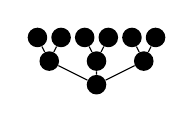
\begin{tikzpicture}[scale=.2]
    \node[circle, scale=0.75, fill] (tid0) at (4.5,1.5){};
    \node[circle, scale=0.75, fill] (tid1) at (1.5,3){};
    \node[circle, scale=0.75, fill] (tid4) at (0.75,4.5){};
    \node[circle, scale=0.75, fill] (tid5) at (2.25,4.5){};
    \draw[](tid1) -- (tid4);
    \draw[](tid1) -- (tid5);
    \node[circle, scale=0.75, fill] (tid2) at (4.5,3){};
    \node[circle, scale=0.75, fill] (tid6) at (3.75,4.5){};
    \node[circle, scale=0.75, fill] (tid7) at (5.25,4.5){};
    \draw[](tid2) -- (tid6);
    \draw[](tid2) -- (tid7);
    \node[circle, scale=0.75, fill] (tid3) at (7.5,3){};
    \node[circle, scale=0.75, fill] (tid8) at (6.75,4.5){};
    \node[circle, scale=0.75, fill] (tid9) at (8.25,4.5){};
    \draw[](tid3) -- (tid8);
    \draw[](tid3) -- (tid9);
    \draw[](tid0) -- (tid1);
    \draw[](tid0) -- (tid2);
    \draw[](tid0) -- (tid3);
  \end{tikzpicture}
\end{center}

However, we will most of the time use a notion where we assume that for a tree sequence $(x_1,x_2,\dots, x_n)$ we have $\forall i \in \left\{ 1,2,\dots,n \right\}x_i\leq i$. This is always possible because we can start a breadth-first search (BFS) at task 0 and assign numbers to the tasks representing the order in which BFS visits the tasks.

\subsection{Labelled and unlabelled intrees}
\label{sec:intrees-labelled-unlabelled}

We can draw such intrees in a very straightforward manner: We draw the root at the bottom and its direct predecessors one level above. For each predecessor, we inductively repeat this procedure to obtain a ``top-to-bottom-description'' of the tree.

Figure \ref{fig:intree-example-task-names-directed-edges} shows an intree (the one given by the sequence $(0,0,1,1,2,3,3,3,6,8)$), where tasks 8 is a requirement for task 6, which itself is -- like task 7, 8 and (indirectly) task 10 -- a requirement for task 3. This figure also illustrates the fact that -- in an intree -- each task is a direct requirement for \emph{at most} one other task.

However, we are mostly interested in the \emph{structure} of the tree, which is why we most of the time omit the labellings of the vertices (i.e. we omit the task names) and rely on a \emph{unlabelled} representation as shown in figure \ref{fig:intree-example-structure-version}. 

\begin{figure}[t]
  \centering
  \begin{subfigure}{.45\textwidth}
    \centering{}
    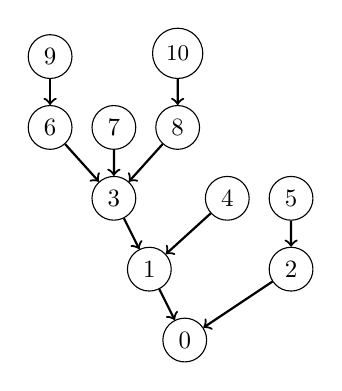
\begin{tikzpicture}[scale=.6, anchor=south]
      \node[circle, scale=0.9, draw] (tid0) at (3,1.5){0};
      \node[circle, scale=0.9, draw] (tid1) at (2.25,3){1};
      \node[circle, scale=0.9, draw] (tid2) at (1.5,4.5){3};
      \node[circle, scale=0.9, draw] (tid7) at (0.15,6){6};
      \node[circle, scale=0.9, draw] (tid9) at (0.15,7.5){9};
      \draw[<-, thick](tid7) -- (tid9);
      \node[circle, scale=0.9, draw] (tid10) at (1.5,6){7};
      \draw[<-, thick](tid2) -- (tid7);
      \draw[<-, thick](tid2) -- (tid10);
      \node[circle, scale=0.9, draw] (tid3) at (3.9,4.5){4};
      \node[circle, scale=0.9, draw] (tid5) at (2.85,6){8};
      \node[circle, scale=0.9, draw] (tid6) at (2.85,7.5){\small 10};
      \draw[<-, thick](tid5) -- (tid6);
      \draw[<-, thick](tid2) -- (tid5);
      \draw[<-, thick](tid1) -- (tid2);
      \draw[<-, thick](tid1) -- (tid3);
      \node[circle, scale=0.9, draw] (tid4) at (5.25,3){2};
      \node[circle, scale=0.9, draw] (tid8) at (5.25,4.5){5};
      \draw[<-, thick](tid4) -- (tid8);
      \draw[<-, thick](tid0) -- (tid1);
      \draw[<-, thick](tid0) -- (tid4);
    \end{tikzpicture}
    \caption{Labelled version with vertex labels and edges drawn as arrows.}
    \label{fig:intree-example-task-names-directed-edges}
  \end{subfigure}
  \quad
  \begin{subfigure}{.45\textwidth}
    \centering{}
    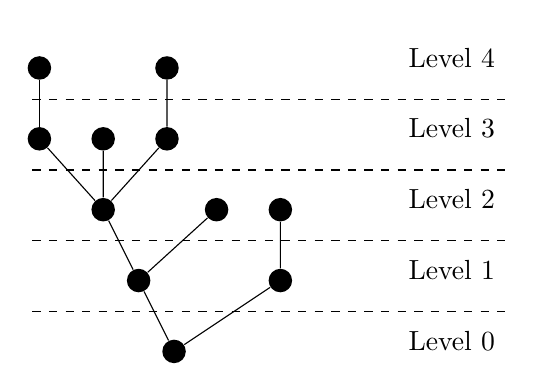
\begin{tikzpicture}[scale=.6, anchor=south]
      \node[circle, scale=0.9, fill] (tid0) at (3,1.5){};
      \node[circle, scale=0.9, fill] (tid1) at (2.25,3){};
      \node[circle, scale=0.9, fill] (tid2) at (1.5,4.5){};
      \node[circle, scale=0.9, fill] (tid7) at (0.15,6){};
      \node[circle, scale=0.9, fill] (tid9) at (0.15,7.5){};
      \draw[](tid7) -- (tid9);
      \node[circle, scale=0.9, fill] (tid10) at (1.5,6){};
      \draw[](tid2) -- (tid7);
      \draw[](tid2) -- (tid10);
      \node[circle, scale=0.9, fill] (tid3) at (3.9,4.5){};
      \node[circle, scale=0.9, fill] (tid5) at (2.85,6){};
      \node[circle, scale=0.9, fill] (tid6) at (2.85,7.5){};
      \draw[](tid5) -- (tid6);
      \draw[](tid2) -- (tid5);
      \draw[](tid1) -- (tid2);
      \draw[](tid1) -- (tid3);
      \node[circle, scale=0.9, fill] (tid4) at (5.25,3){};
      \node[circle, scale=0.9, fill] (tid8) at (5.25,4.5){};
      \draw[](tid4) -- (tid8);
      \draw[](tid0) -- (tid1);
      \draw[](tid0) -- (tid4);
      % level separators
      \draw[dashed] (0, 2.6) -- +(10, 0) node[below left, yshift=-.125cm]{Level 0};
      \draw[dashed] (0, 4.1) -- +(10, 0) node[below left, yshift=-.125cm]{Level 1};
      \draw[dashed] (0, 5.6) -- +(10, 0) node[below left, yshift=-.125cm]{Level 2};
      \draw[dashed] (0, 7.1) -- +(10, 0) node[below left, yshift=-.125cm]{Level 3};
      \draw[      ] (0, 8.6)    +(10, 0) node[below left, yshift=-.125cm]{Level 4};
    \end{tikzpicture}
    \caption{Unlabelled version without arrows, edges are implicitly directed towards the root.}
    \label{fig:intree-example-structure-version}
  \end{subfigure}
  \caption{Graphical representation of an intree ($(0,0,1,1,2,3,3,3,6,8)$) with 5 levels (numbered 0 to 4). All edges are implicitly directed towards the root, which is drawn at the bottom of the tree. Most of the time, the \emph{structure} of the tree is enough, so we will omit vertex names most of the time.}
  \label{fig:intrees-introductory-explanation}
\end{figure}

The mathematical concept behind unlabelled trees can be described by the notion of \emph{isomorphisms}.

\begin{definition}[Intree isomorphism]
  We call two intrees $I_1$ and $I_2$ \emph{isomorphic}, if there exists a bijective function that maps vertices of $I_1$ onto vertices of $I_2$ such that $(v,t)$ is an edge in $I_1$ if and only if $(f(v), f(t))$ is an edge in $I_2$ and the root of $I_1$ is mapped onto the root of $I_2$.
\end{definition}

\emph{Remark:} The above definition of isomorphisms is somewhat non-standard in the sense that usually isomorphisms are defined for undirected trees. For this work, we restrict ourselves onto our definition (except where explicitly stated otherwise).

As an example for isomorphic intrees, consider $(0,0,1,1,2,3,3,3,6,8)$, $(0,1,2,3,0,5,1,2,2,9)$ and $(0,1,0,3,3,4,4,7,4,9)$.

Since we are using a notion of intrees as aforementioned (i.e. with $\forall i \in \left\{ 1,2,\dots,n \right\}.\ x_i \leq i$), this means that there are $n!$ possibilities for tree sequences with exactly $n$ tasks. On the other hand, there are less (distinct) intrees of size $n$:

\begin{theorem}
  Let $T_n$ denote the number of intrees containing $n$ tasks. Then,
  \begin{equation*}
    T_n \sim C\cdot r^{-n}\cdot n^{-1.5} 
    \quad \text{ as } n\rightarrow \infty,
  \end{equation*}
  where $C=0.4399237\dots$ and $r=0.3383219\dots$.
\end{theorem}

\begin{proof}
  See \cite{asymptotic_enum_odlyzko}.
\end{proof}

The first values for $T_n$ are $0, 1, 1, 2, 4, 9, 20, 48, 115, 286, 719, 1842, 4766, 12486, 32973, \dots$ \cite{oeisrootedtrees}.

In some cases it is useful to consider only intrees with a certain number of \emph{leaves}. If we consider the set of all intrees with $n$ tasks it is clear that \emph{all but one} intree have more than one leaf (the only intree having exactly one leaf is a chain of $n$ tasks). For us, especially the number of intrees with at least 4 leaves might be of interest \footnote{Because all other intrees -- with 3 or less leaves -- are trivially optimally scheduled by HLF (see section \ref{sec:intro-two-scheduling-strategies}).}. Moreover, an optimal schedule for an intree whose root has exactly one predecessor (meaning that the degree of the root is 1 or -- more mathematically -- $\deg (0) = 1$) looks the same as if we omitted the root and scheduled it after the whole intree \emph{without} the root. Table \ref{tab:number-of-intrees-summary} sums up the number of intrees fulfilling the respective properties.

\begin{table}[th]
  \centering
  \begin{tabular}[ht]{r|cccccccccccccc}
    Tasks & 3 & 4 & 5 & 6 & 7 & 8 & 9 & 10 & 11 & 12 & 13 & 14 & 15 \\
    \hline
    Intrees & 2 & 4 & 9 & 20 & 48 & 115 & 286 & 719 & 1842 & 4766 & 12486 & 32973 & 87811 \\
    $\geq 4$ leaves & 0& 0& 1& 5& 20& 67& 207& 595& 1655& 4494& 12101& 32443& 87097 \\
    $\deg (0) > 1$ & 1 & 2 & 5 & 11 & 28 & 67 & 171 & 433 & 1123 & 2924 & 7720 & 20487 & 54838 \\
    $\geq 4$ leaves; $\deg{0} > 1$ & 0 & 0 & 1 & 4 & 15 & 47 & 140 & 388 & 1060 & 2839 & 7607 & 20342 & 54654 \\
  \end{tabular}
  \caption{Number of intrees with a certain number of tasks and certain properties (namely if they have at least 4 leaves and/or if their root has more than one predecessor).}
  \label{tab:number-of-intrees-summary}
\end{table}

\subsection{Interpretation as dependency graphs}
\label{sec:intrees-interpreted-as-dependency-graphs}

Those intrees can naturally be used to describe dependencies between different tasks, as long as each task is the requirement for \emph{at most one} other task. Each vertex in an intree then represents a task. If $t_1$ is a (direct) predecessor of $t_2$, this means that the task associated with $t_1$ must be executed before the task associated with $t_2$. Since we represent tasks by vertices, we will often use the terms task and vertex interchangeably.

\todo{Vielleicht ein Beispiel aus der echten Welt.}

\begin{definition}[Ready tasks]
  Let $I$ be an intree of tasks (represented by vertices) and. If $t$ is a leaf of $I$, we call the corresponding task (resp. -- for simplicity -- the whole vertex) \emph{ready}.
\end{definition}

The intree $(0,0,1,1,2,3,3,3,6,8)$ (see figure \ref{fig:intree-example-task-names-directed-edges}) has the ready tasks 4, 5, 7, 9 and 10.

\subsection{Extension to in-forests}
\label{sec:intrees-extension-to-forests}

It is worth mentioning that -- for our needs -- there is a straightforward extension of intrees to in-forests for our scenario. In-forests are graphs whose components are all intrees. To convert an in-forest to an intree, we simply add an auxiliary new root and connect all roots of the intrees within the in-forest to the new root. This way, we clearly obtain a new intree.

\begin{figure}[th]
  \centering
  \begin{subfigure}{.45\textwidth}
    \centering
    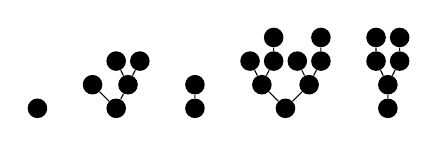
\begin{tikzpicture}[scale=.2, anchor=south]
      \begin{scope}[xshift=-2cm]
        \begin{scope}[xshift=-2cm]
          \node[circle, scale=0.75, fill] (tid1) at (0.75,3){};
        \end{scope}
        \node[circle, scale=0.75, fill] (tid2) at (3.75,3){};
        \node[circle, scale=0.75, fill] (tid6) at (2.25,4.5){};
        \node[circle, scale=0.75, fill] (tid7) at (4.5,4.5){};
        \node[circle, scale=0.75, fill] (tid12) at (3.75,6){};
        \node[circle, scale=0.75, fill] (tid13) at (5.25,6){};
      \end{scope}
      \draw[](tid7) -- (tid12);
      \draw[](tid7) -- (tid13);
      \draw[](tid2) -- (tid6);
      \draw[](tid2) -- (tid7);
      \node[circle, scale=0.75, fill] (tid3) at (6.75,3){};
      \node[circle, scale=0.75, fill] (tid8) at (6.75,4.5){};
      \draw[](tid3) -- (tid8);
      \begin{scope}[xshift=2cm]
        \node[circle, scale=0.75, fill] (tid4) at (10.5,3){};
        \node[circle, scale=0.75, fill] (tid9) at (9,4.5){};
        \node[circle, scale=0.75, fill] (tid14) at (8.25,6){};
        \node[circle, scale=0.75, fill] (tid15) at (9.75,6){};
        \node[circle, scale=0.75, fill] (tid20) at (9.75,7.5){};
        \draw[](tid15) -- (tid20);
        \draw[](tid9) -- (tid14);
        \draw[](tid9) -- (tid15);
        \node[circle, scale=0.75, fill] (tid10) at (12,4.5){};
        \node[circle, scale=0.75, fill] (tid16) at (11.25,6){};
        \node[circle, scale=0.75, fill] (tid17) at (12.75,6){};
        \node[circle, scale=0.75, fill] (tid21) at (12.75,7.5){};
        \draw[](tid17) -- (tid21);
        \draw[](tid10) -- (tid16);
        \draw[](tid10) -- (tid17);
        \draw[](tid4) -- (tid9);
        \draw[](tid4) -- (tid10);
        \begin{scope}[xshift=2cm]
          \node[circle, scale=0.75, fill] (tid5) at (15,3){};
          \node[circle, scale=0.75, fill] (tid11) at (15,4.5){};
          \node[circle, scale=0.75, fill] (tid18) at (14.25,6){};
          \node[circle, scale=0.75, fill] (tid22) at (14.25,7.5){};
          \draw[](tid18) -- (tid22);
          \node[circle, scale=0.75, fill] (tid19) at (15.75,6){};
          \node[circle, scale=0.75, fill] (tid23) at (15.75,7.5){};      
        \end{scope}
      \end{scope}
      \draw[](tid19) -- (tid23);
      \draw[](tid11) -- (tid18);
      \draw[](tid11) -- (tid19);
      \draw[](tid5) -- (tid11);
    \end{tikzpicture}
    \caption{Original in-forest (each component is a separate intree).}
  \end{subfigure}
  \quad
  \begin{subfigure}{.45\textwidth}
    \centering
    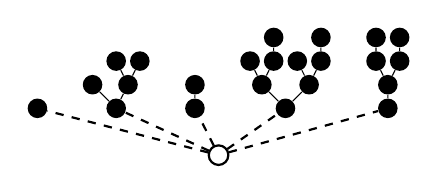
\begin{tikzpicture}[scale=.2, anchor=south]
      \node[circle, scale=0.75, draw, thick] (tid0) at (8.25,0){};
      \begin{scope}[xshift=-2cm]
        \begin{scope}[xshift=-2cm]
          \node[circle, scale=0.75, fill] (tid1) at (0.75,3){};
        \end{scope}
        \node[circle, scale=0.75, fill] (tid2) at (3.75,3){};
        \node[circle, scale=0.75, fill] (tid6) at (2.25,4.5){};
        \node[circle, scale=0.75, fill] (tid7) at (4.5,4.5){};
        \node[circle, scale=0.75, fill] (tid12) at (3.75,6){};
        \node[circle, scale=0.75, fill] (tid13) at (5.25,6){};
      \end{scope}
      \draw[](tid7) -- (tid12);
      \draw[](tid7) -- (tid13);
      \draw[](tid2) -- (tid6);
      \draw[](tid2) -- (tid7);
      \node[circle, scale=0.75, fill] (tid3) at (6.75,3){};
      \node[circle, scale=0.75, fill] (tid8) at (6.75,4.5){};
      \draw[](tid3) -- (tid8);
      \begin{scope}[xshift=2cm]
        \node[circle, scale=0.75, fill] (tid4) at (10.5,3){};
        \node[circle, scale=0.75, fill] (tid9) at (9,4.5){};
        \node[circle, scale=0.75, fill] (tid14) at (8.25,6){};
        \node[circle, scale=0.75, fill] (tid15) at (9.75,6){};
        \node[circle, scale=0.75, fill] (tid20) at (9.75,7.5){};
        \draw[](tid15) -- (tid20);
        \draw[](tid9) -- (tid14);
        \draw[](tid9) -- (tid15);
        \node[circle, scale=0.75, fill] (tid10) at (12,4.5){};
        \node[circle, scale=0.75, fill] (tid16) at (11.25,6){};
        \node[circle, scale=0.75, fill] (tid17) at (12.75,6){};
        \node[circle, scale=0.75, fill] (tid21) at (12.75,7.5){};
        \draw[](tid17) -- (tid21);
        \draw[](tid10) -- (tid16);
        \draw[](tid10) -- (tid17);
        \draw[](tid4) -- (tid9);
        \draw[](tid4) -- (tid10);
        \begin{scope}[xshift=2cm]
          \node[circle, scale=0.75, fill] (tid5) at (15,3){};
          \node[circle, scale=0.75, fill] (tid11) at (15,4.5){};
          \node[circle, scale=0.75, fill] (tid18) at (14.25,6){};
          \node[circle, scale=0.75, fill] (tid22) at (14.25,7.5){};
          \draw[](tid18) -- (tid22);
          \node[circle, scale=0.75, fill] (tid19) at (15.75,6){};
          \node[circle, scale=0.75, fill] (tid23) at (15.75,7.5){};      
        \end{scope}
      \end{scope}
      \draw[](tid19) -- (tid23);
      \draw[](tid11) -- (tid18);
      \draw[](tid11) -- (tid19);
      \draw[](tid5) -- (tid11);
      \draw[dashed, thick](tid0) -- (tid1);
      \draw[dashed, thick](tid0) -- (tid2);
      \draw[dashed, thick](tid0) -- (tid3);
      \draw[dashed, thick](tid0) -- (tid4);
      \draw[dashed, thick](tid0) -- (tid5);
    \end{tikzpicture}
    \caption{Adding a new root that is connected with all intrees' roots.}
  \end{subfigure}
  \caption{Converting an in-forest to an intree.}
  \label{fig:in-forest-to-intree}
\end{figure}

To manipulate intrees, we define some non-standard notation that is, however, very convenient and should be easily understandable.

%%% Local Variables:
%%% TeX-master: "../thesis.tex"
%%% End: 